\chapter{开始学习Ren'Py}

\begin{ChapterGoals}
    \begin{itemize}
        \item \FZFangSong 使用DDLC Mod中文模版创造一个项目;
        \item \FZFangSong 学会使用say语句;
        \item \FZFangSong 学会使用show、hide、scene语句;
        \item \FZFangSong 学会使用play、stop语句;
        \item \FZFangSong 学会使用menu语句;
    \end{itemize}
\end{ChapterGoals}

要建造一个属于我们的房屋,就必须要先打地基、搭框架。如果说Ren'Py是项目的地基,那么Mod模板就是一个框架,我们可以在这个框架中快速地放置门、窗等,还可以自定义这个框架,而不必先调制水泥,然后从地基一步步开始。通过模版,我们可以省去很多步骤。本章我们将在DDLC Mod中文模版的基础上将对Ren'Py进行初步学习。

\section{准备开发环境}
DDLC Mod模板是由GanstaKingofSA编写的一个方便开发Mod的模板。imgradeone对其进行了本土化。目前,DDLC Mod中文模板主要流行三个大版本:1.0版本,2.0版本(即Next分支)与4.0版本(即Future分支)。
\begin{itemize}
    \item 1.0 版本仅支持 Ren'Py 6,且没有什么特别功能;
    \item 2.0 版本增加支持了 Ren'Py 7、Android 移植等功能;
    \item 4.0 版本增加支持了 Ren'Py 8 与 Python 3,增加额外屏幕(Extra Screen)功能等,但稳定性存疑。
\end{itemize}

本书将使用 2.0 版本进行讲解。

\subsection{下载DDLC Mod中文模版}

\begin{figure}[htb]
    \centering
    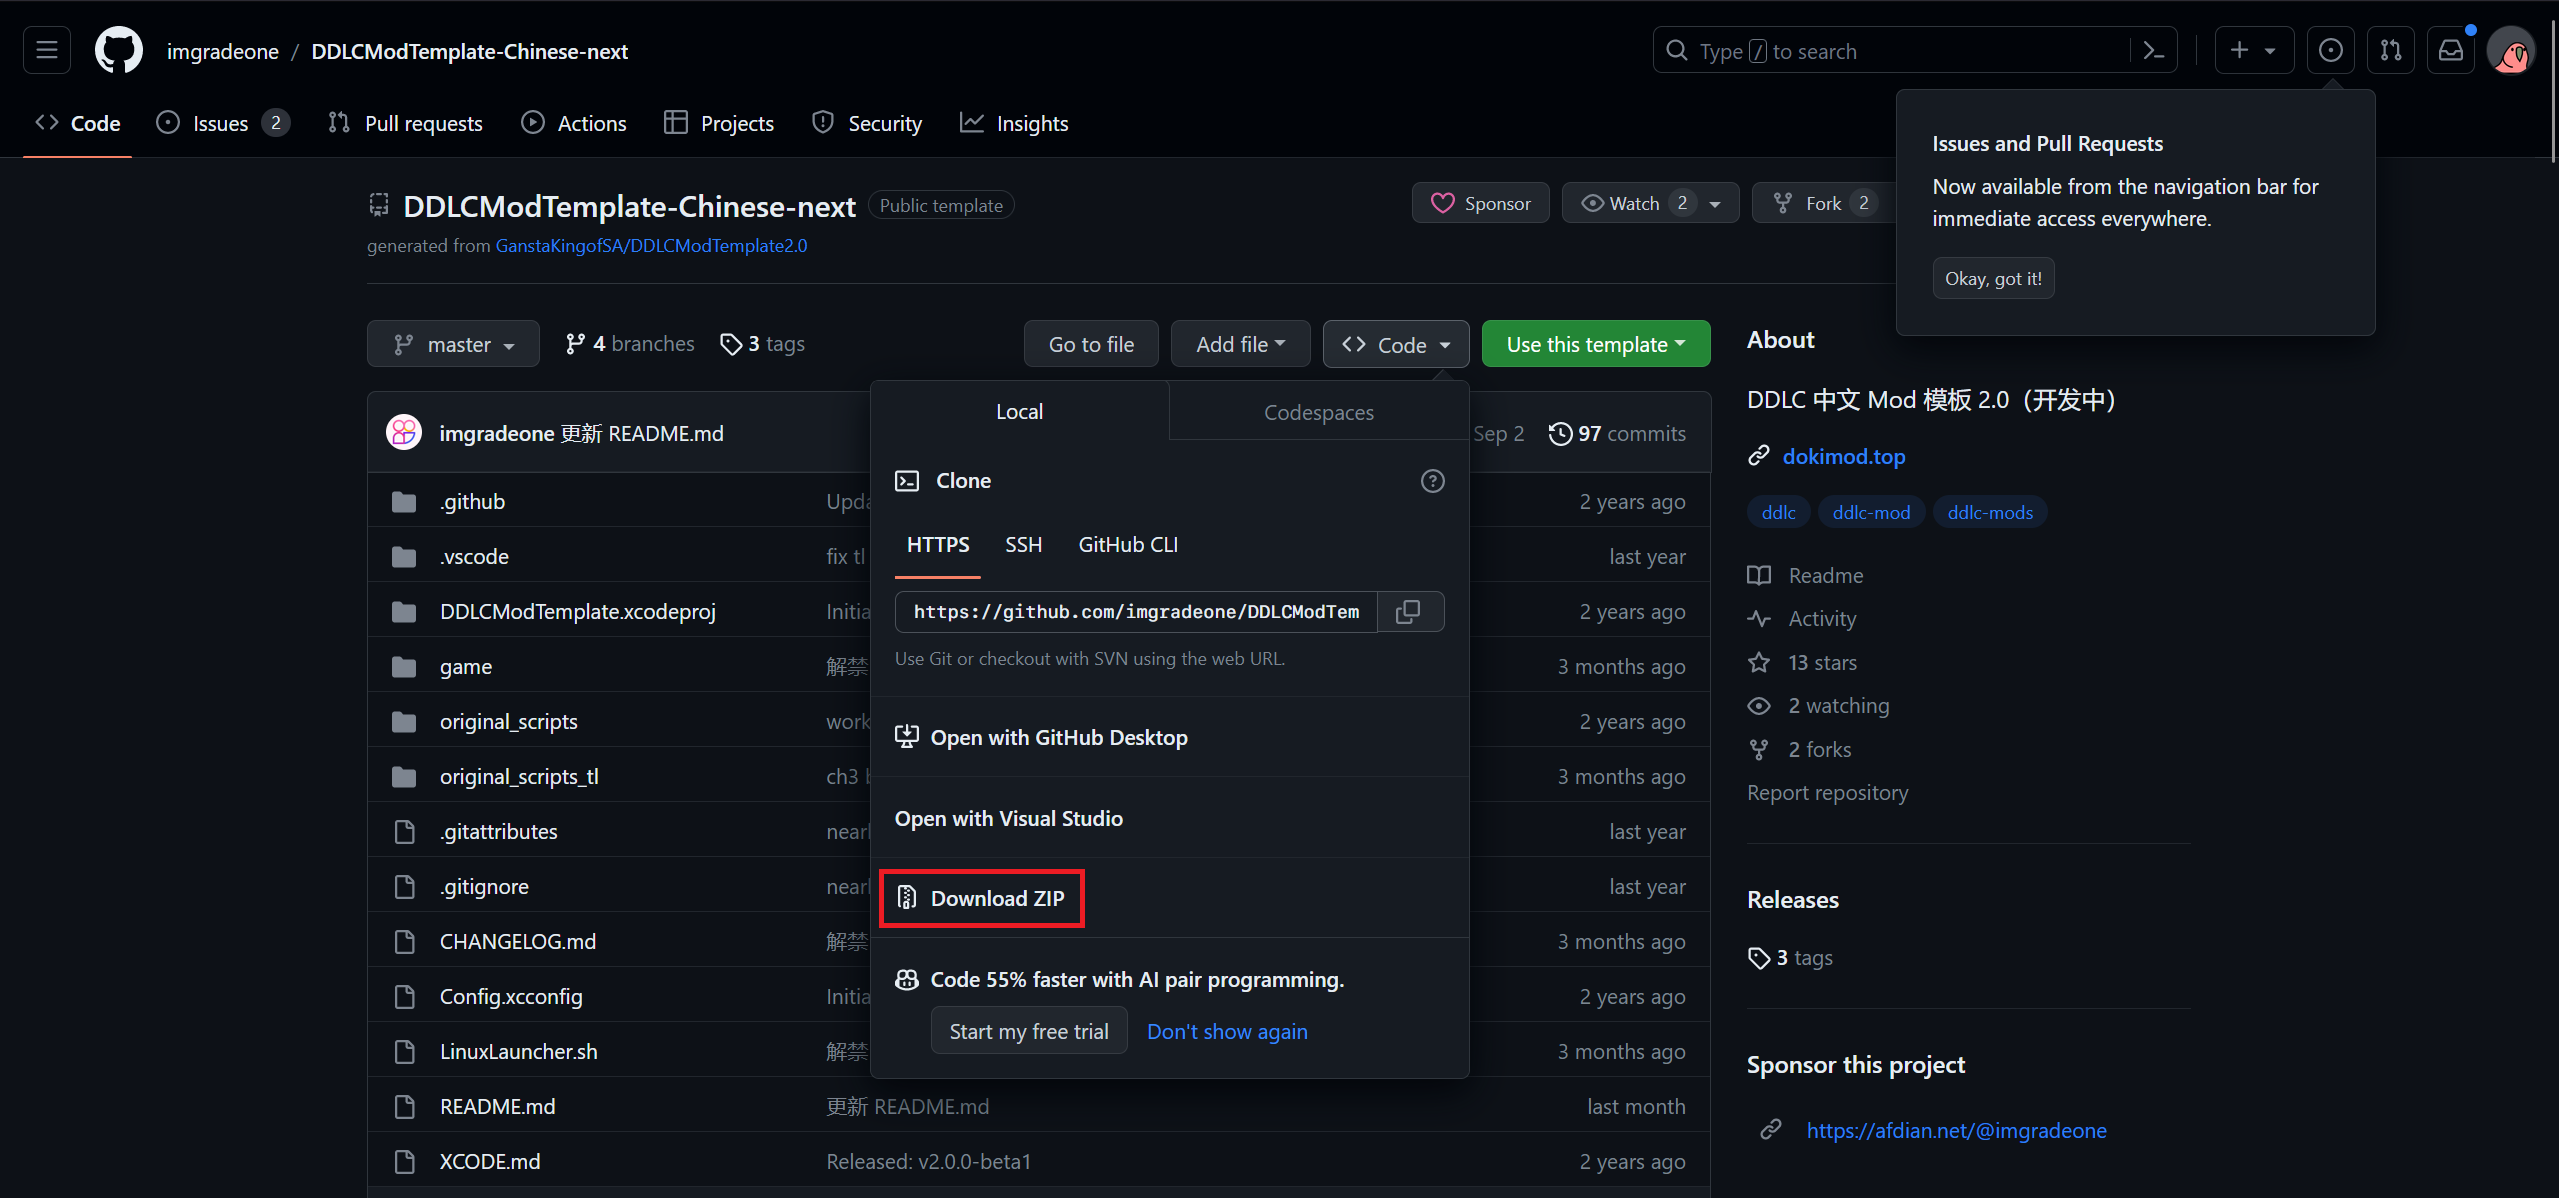
\includegraphics[scale=.15]{Pictures/2/2.1/2.1.1}
    \caption{项目页面}
    \label{fig:3.1.1.1}
\end{figure}
使用任意浏览器打开github.com/imgradeone/DDLCModTemplate-Chinese-next,将压缩包下载下来(如图\ref{fig:3.1.1.1}所示)。

下载完成后解压至在第\ref{sec:2.2.1}节中您下载的Ren'Py SDK的目录下。完成该步骤后,您的Ren'Py SDK中项目一栏应出现DDLCModTemplate-Chinese-next。

从 https://ddlc.moe/中下载原版DDLC,打开压缩包后将DDLC-1.1.1-pc/game/下的audio.rpa、images.rpa、fonts.rpa解压至Mod中文模板下的game/文件夹中。此时,Mod中文模板下的game/文件夹结构应如图\ref{fig:3.1.1.2}所示。

\begin{figure}[htbp]
    \centering
    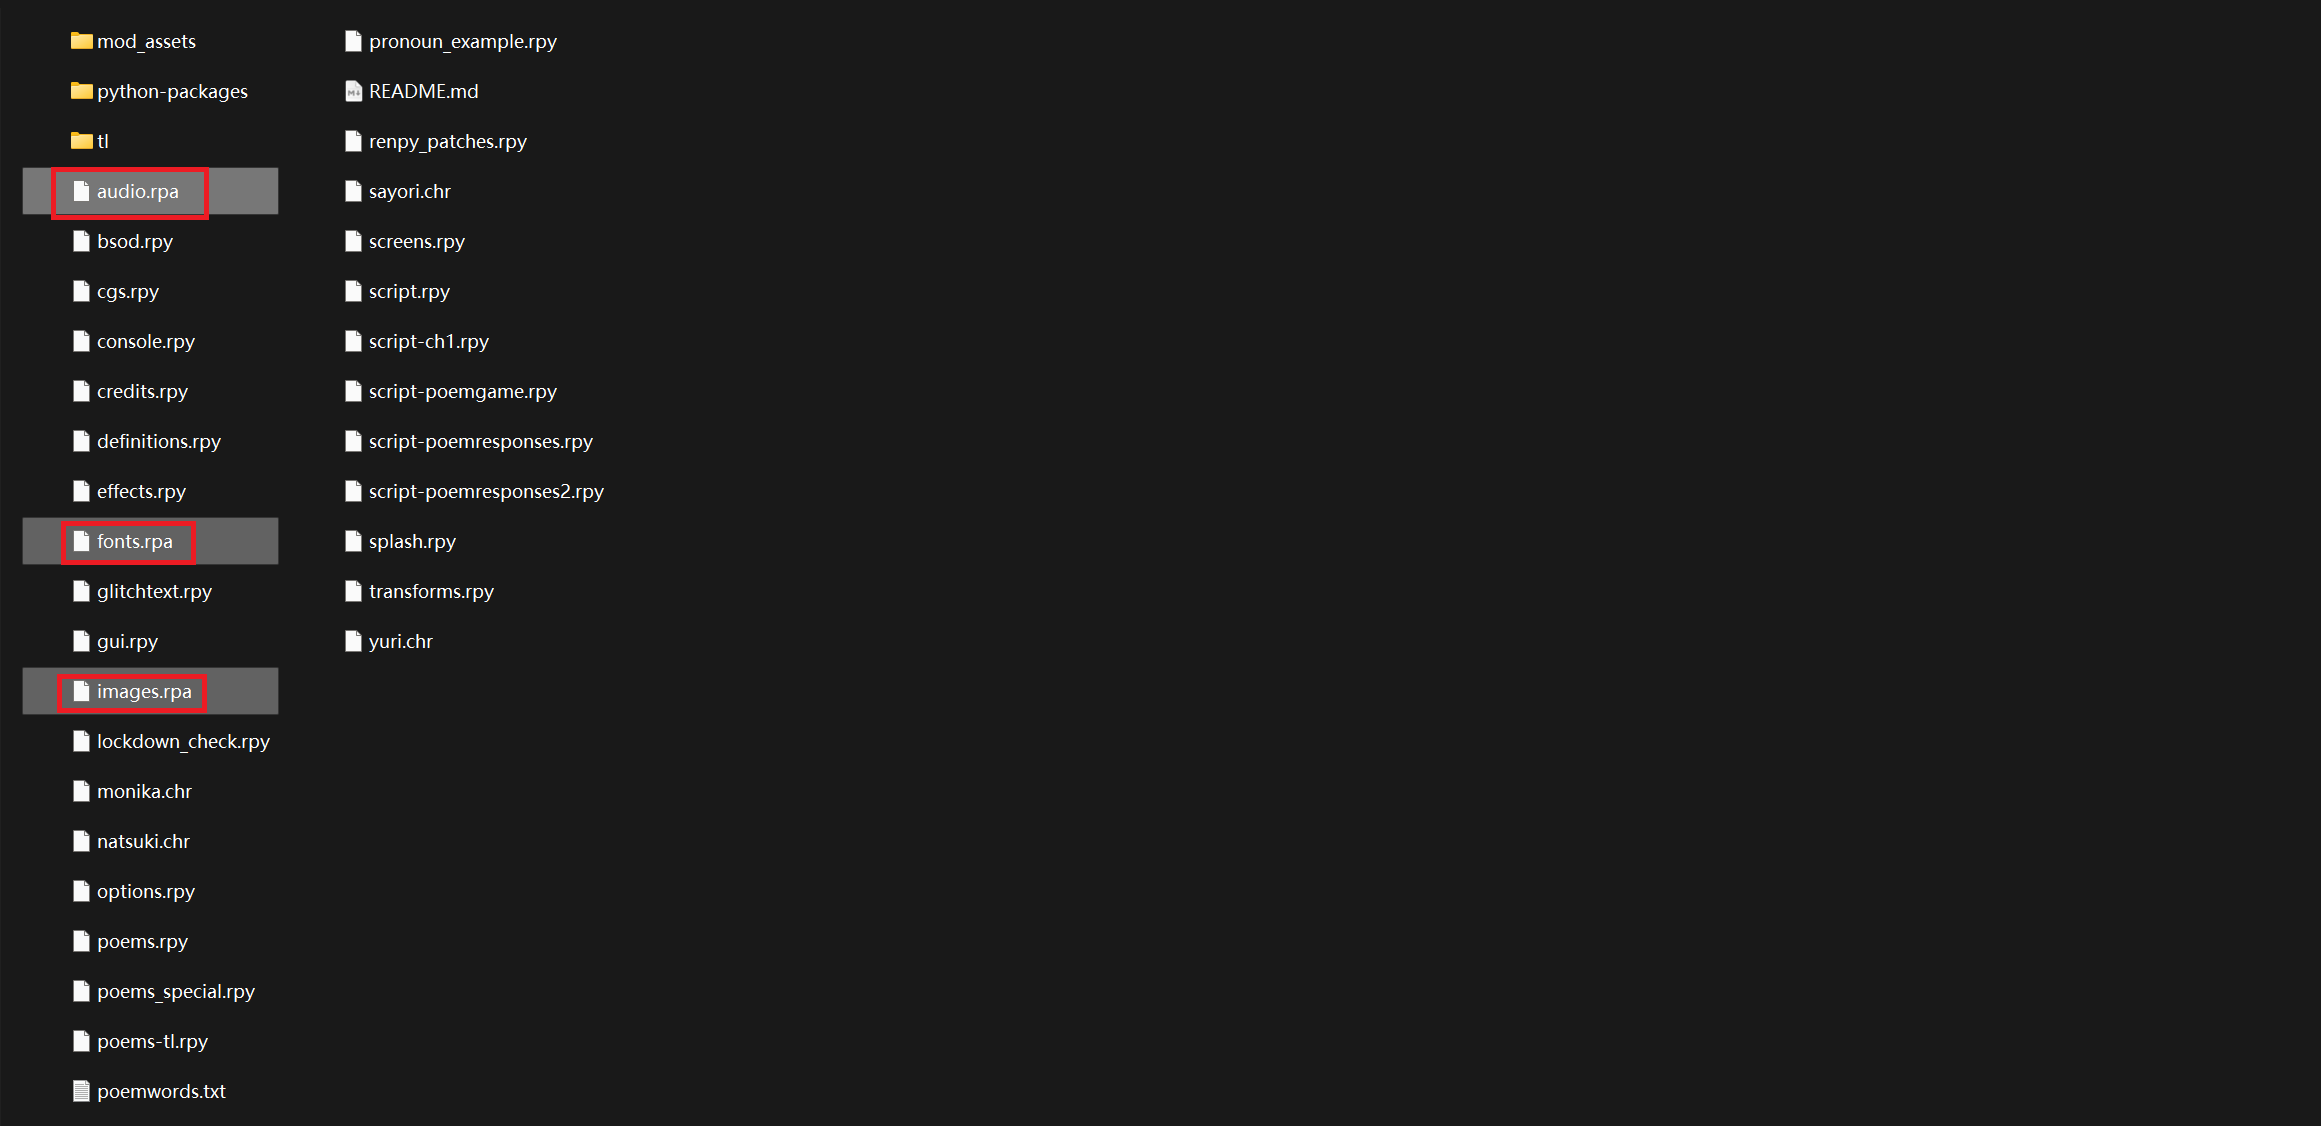
\includegraphics[scale=.2]{Pictures/2/2.1/2.1.2}
    \caption{项目结构}
    \label{fig:3.1.1.2}
\end{figure}

至此,您就完成了准备工作的第一部分———下载DDLC Mod中文模板并完成配置。

\subsection{配置文本编辑器}
有了Mod中文模板,我们还需要一个趁手的编辑器。你大可选择记事本,不过Ren'Py SDK也为我们提供了两种文本编辑器:Visual Studio Code和Atom。本书将以Visual Studio Code为例配置文本编辑器。

打开Ren'Py SDK,点击右下角的设置。在一般选项卡中选择文本编辑器,此时点击第一个选项Visual Studio Code。Ren'Py会开始下载Visual Studio Code与Ren'Py插件。耐心等待一段时间后,会返回到设置界面。此时点击返回,点击DDLCModTemplate-Chinese-next,点击编辑选项卡下的“打开项目”会打开Visual Studio Code(如图\ref{fig:3.1.2.1}所示)。

\begin{figure}[htbp]
    \centering
    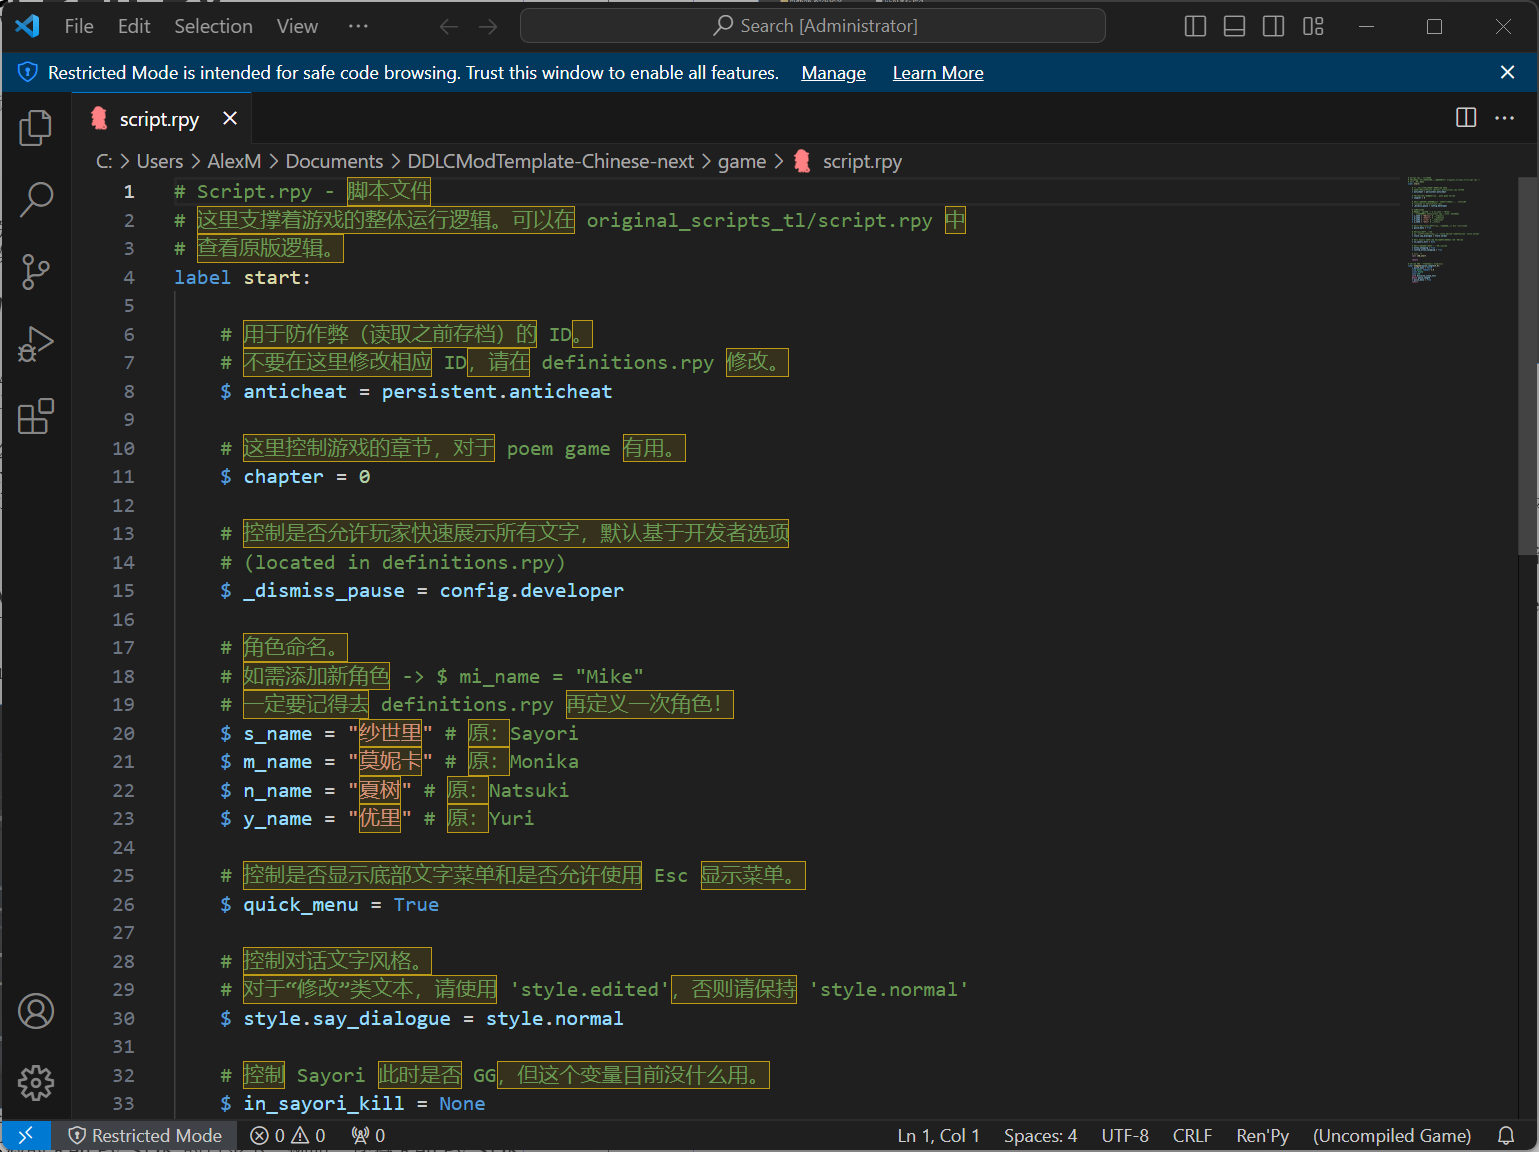
\includegraphics[scale=.4]{Pictures/2/2.1/2.1.3}
    \caption{Visual Studio Code}
    \label{fig:3.1.2.1}
\end{figure}

此时点击扩展选项卡,输入Chinese,点击第一个搜索结果中的Install。此时右下角会弹出提示框询问是否切换语言并重启。点击Change Language and Restart。重启后 Visual Studio Code 就会切换成中文。

打开Ren'Py SDK,选中DDLCModTemplate-Chinese-next,点击编辑文件选项卡中的“打开项目”,Ren'Py SDK会自动帮我们打开Visual Studio Code并定位到本项目。

随后,展开左侧资源管理器中的“game”文件夹,打开script-ch1.rpy文件。保留文件第一行,删除其他内容即可。至此,我们就正式完成了开发的准备工作。

\begin{figure}[htbp]
    \centering
    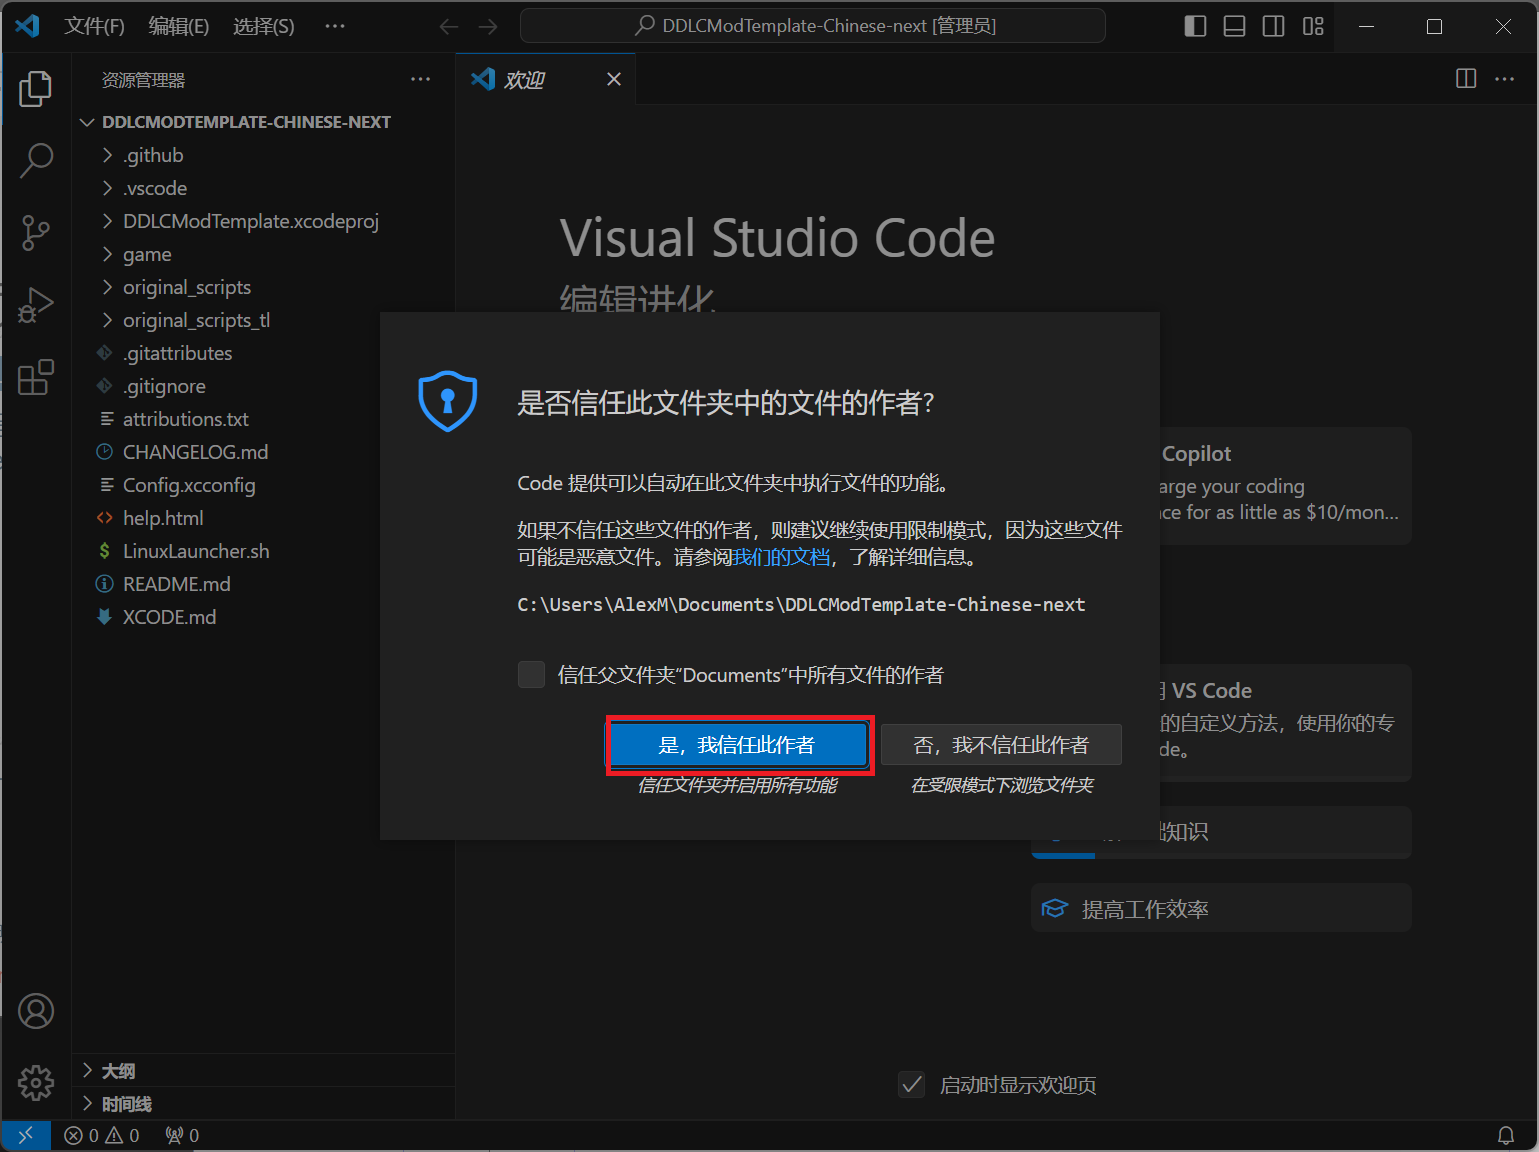
\includegraphics[scale=.4]{Pictures/2/2.2/2.2.1}
    \caption{Visual Studio Code}
    \label{fig:3.1.2.2}
\end{figure}

\begin{Comment}
    若您打开 Visual Studio Code 时出现如图\ref{fig:3.1.2.2}所示的提示框,请点击“是,我信任此作者”。
\end{Comment}

\subsection{设置您的游戏}
做好了上述准备工作,我们还有最后一项任务需要完成————配置你的游戏设置。游戏设置关系到游戏的正常运行、存读档。现在,在Visual Studio Code左侧资源管理器中game目录下的options.rpy文件

现在,将根据下表,将原有内容替换或进行配置。




\section{进入Ren'Py世界}
在Ren'Py的世界里,剧本与视觉内容都围绕着代码展开。要编写脚本,我们就必须先学习Ren'Py的语法。
\subsection{say语句}\label{subsec:3.2.1}
say语句是一个十分重要的语法,它可以让视觉小说角色拥有对话的能力。不过不用担心,say
语句的语法十分简单。

还记得上一课我们打开的script-ch1.rpy吗?现在另起一行,按下 Tab 键(或打四个空格,不过Visual Studio Code会自动为我们将Tab转化为空格),输入以下代码片段:

\begin{lstlisting}
    "快到学园祭了"
    m "各位!我们得开始准备了!"
\end{lstlisting}

\begin{Warning}
您必须使用英文引号来包住文字。另外,请务必注意缩进问题,错误的缩进将会导致代码运行失败。
\end{Warning}

这是一段非常简单的Ren'Py代码,它只包含文字,不显示任何图像或播放任何音效。现在,切换回Ren'Py SDK,点击启动项目,开始游戏,您应该会看到一行旁白以及莫妮卡的一行对话。

在理解以上基础内容之后,我们可以添加更多对话。不过在那之前,你得先了解 say 语句的基础语法:

\begin{lstlisting}[numbers=none]
<角色名> "<说话内容>"
\end{lstlisting}


此处的角色名应对应下列表格:

\begin{center}
    \tablehead{
    \hline
    角色名 & 对应角色 \\
    \hline
    }
    \tabletail{\hline}
    \tablelasttail{\hline}
    \begin{supertabular}{|c|c|}
        \hline
        m & 莫妮卡(Monika)\\
        s & 纱世里(Sayori)\\
        y & 优里(Yuri)\\
        n & 夏树(Natsuki)\\
        mc & 主人公(Main Character)\\
        留空 & 旁白(Narrator)\\
        \hline
    \end{supertabular}
    \captionof{table}{角色名表格}
\end{center}

现在,尝试理解下列代码并运行:

\begin{lstlisting}[caption=scipt-ch1.rpy, label={lst:2.1}]
# Chapter 0
label ch0_start:
    "快到学园祭了。"
    m "各位!我们得开始准备了! "
    s "好耶!!!! "
    n "啊,我都等不及学园祭了。"
    n "肯定会很棒的! "
    y "..."
    return
\end{lstlisting}

在Ren'Py中,我们使用脚本标签(label)来声明代码块。(关于脚本标签的知识,我们将会在后续内容进行详细讲解)。通常,在Ren'Py项目中都含有一个名为start的脚本标签。但是在DDLC Mod 模板中,script.rpy文件已经为我们声明好了start脚本标签。在本段代码中,script-ch1.rpy包含以下几件事:

\begin{itemize}
    \item 第一行的注释;
    \item 创造一个名为ch0\_start的代码块;
    \item say语句创造对话;
    \item return语句返回到上级。
\end{itemize}

\begin{Comment}
在Ren'Py中,我们使用与Python相同的“\#”来表示本行为注释。注释行的内容将不会被 Ren'Py或Python执行。
\end{Comment}

当我们需要在对话中提及玩家的名字、需要将某些内容突出显示或对某部分文字需要进行特殊处理时,应当怎么办呢?读代码\ref{lst:2.2},尝试理解其用法,并在游戏中运行,看看与自己的猜测是否相同。

\begin{lstlisting}[caption=scipt-ch1.rpy, label={lst:2.2}]
# Chapter 0
label ch0_start:
    "{cps=20} 快到 {b} 学园祭 {/b} 了。{/cps}{w=.5}{nw}"
    m "各位!我们得开始准备了!"
    s "好耶!!!!"
    n "啊,我都等不及学园祭了。"
    n "肯定会很棒的!"
    y "..."
    m "那么,是时候来进行分工了。"
    m "[player],你想要做什么?"
    return
\end{lstlisting}

\begin{ExtraKnowledge}
player是一个记录了玩家名字的变量。不理解变量是什么?没关系,本书将在后面为您介绍变量的性质与作用。在这里,您只需要知道当需要提及玩家名字时使用player变量即可。

您或许也注意到了\{/cps\}和\{/b\}。这是对前面cps标签和bold标签的闭合,代表着其适用范围仅为自身标签与闭合标签内的所有文字。
\end{ExtraKnowledge}

不难发现,当需要使用变量时,我们只需要使用中括号将变量名括住。当我们需要将某段文字进行加粗等操作,可以对文字打上标签(既花括号)。若需要在对话中使用这些字符,则需要连续出现两次。如在代码中要出现花括号,则应该使用\{\{\}\}代替\{\}

以下为常用的文字标签:
\begin{center}
    \tablehead{
    \hline
    标签 & 作用\\
    \hline
    }
    \tabletail{\hline}
    \tablelasttail{\hline}
    \begin{supertabular}{|c|c|}
        \hline
        \{b\} & 将文本渲染为粗体 \\
        \hline
        \{i\} & 将文本渲染为斜体 \\
        \hline
        \{color=<16进制颜色>\} & 将文本渲染为指定颜色 \\
        \hline
        \{font=<字体文件>\} & 使用指定字体渲染文本 \\
        \hline
        \{cps=<数字>\} & 以指定速度渲染文本 \\
        \hline
        \{nw\} & 不等待用户操作,渲染完本行文字后立即渲染下一行 \\
        \hline
        \{w=<数字>\} & 等待一定秒数后或用户操作后继续渲染文本 \\
        \hline
    \end{supertabular}
    \captionof{table}{常用文本处理标签}
    \label{table:3.2.1}
\end{center}

\subsection{show、hide、scene语句}

在\ref{subsec:3.2.1}课中,我们学习了如何在视觉小说中编写对话。但现在有一个很大的问题⸺没有图像。在视觉小说中,视觉便是重点。在本课中,我们将学习如何在视角小说中显示图像。

\subsubsection{show语句}

show语句是Ren'Py游戏中的一个重要语句。它可以让一个图像显示在屏幕上。这个图像可以是背景,也可以是角色。

还记得上一课中的代码吗?请阅读以下代码并尝试理解,在Ren'Py中运行,看看运行实际效果与自己的理解是否正确。

\begin{lstlisting}[caption=script-ch1.rpy, label={lst:2.3}]
# Chapter 0
label ch0_start:
    show bg club_day
    "{cps=20}快到{b}学园祭{/b}了。{/cps}{w=.5}{nw}"
    show monika 1a at t41 zorder 1
    m "各位!我们得开始准备了!"
    show sayori 1a at t42 zorder 1
    s "好耶!!!!"
    show natsuki 1a at t43 zorder 1
    n "啊,我都等不及学园祭了。"
    n "肯定会很棒的!"
    show yuri 1a at t44 zorder 1
    y "..."
    m "那么,是时候来进行分工了。"
    m "[player],你想要做什么?"
    return
\end{lstlisting}

由此可知,show语句的基础语法为:
\begin{lstlisting}[numbers=none]
show <图片名称> <附加参数>
\end{lstlisting}

在游戏中,图片名称可以大致分为三类:
\begin{itemize}
    \item 角色立绘
    \item 背景立绘
    \item 毛刺(Glitch)立绘
\end{itemize}

\paragraph{角色立绘}\label{para:3.2.2.1}

对于角色立绘,图片名称的组成为:
\begin{lstlisting}[numbers=none]
<角色名> <立绘编号>
\end{lstlisting}

DDLC原版中,一个显示在屏幕上的角色立绘可以分为两个部分:身体姿势与面部表情。(实际上,DDLC中的立绘为三个部分:左侧身体姿势、右侧身体姿势、面部表情)

模版中已经将所有可能的身体姿势为我们组合好了。除优里外的所有角色都有五个姿势(1-4为正常站位,5为特殊站位),而优里只有4个姿势(1-3为正常站位,4为特殊站位)。

面部表情使用英文小写字母来表示(请注意,不是所有的角色的面部表情都表示到z。如莫妮卡的面部表情就远少于夏树的面部表情)。

同时,除莫妮卡外的所有角色都可以使用日常服,只需要在身体姿势后加上b即可使用日常服。如:1b

对于角色立绘的列举,您可以前往 \url{https://docs.dokimod.top/pages/0a59cf/} 与 \url{https://ddlc-modding.fandom.com/wiki/Expressions_and_Poses} 查看。


\paragraph{毛刺立绘}

毛刺立绘则是指在二周目出现的大多数“错误”立绘,如错乱的莫妮卡等。
对于毛刺立绘,其图片名称的构成为:
\begin{lstlisting}[numbers=none]
<角色名> <毛刺编号>
\end{lstlisting}

\begin{Warning}
    我们不建议您使用毛刺立绘,因为这对于某些厨可能极不友好。
\end{Warning}

一般来说,毛刺编号为glitch。但是请注意,莫妮卡的毛刺立绘编号为g1与g2;夏树的毛刺立绘则包括ghost\_blood、ghost1、ghost2等。

若要使用优里的自杀立绘,则毛刺编号为stab\_+数字1-6。

\paragraph{背景立绘}

对于背景立绘,其图片名称构成为:
\begin{lstlisting}
bg <背景编号>
\end{lstlisting}

背景编号即意义可以在definitions.rpy文件中找到。这里不再进行过多叙述。

\begin{ExtraKnowledge}
通常我们不使用show来显示背景,而是使用scene。对于scene的详细介绍请看第\ref{subsubsec:3.2.2.3}课。
\end{ExtraKnowledge}

\paragraph{附加参数}

对于附加参数,常用的有:
\begin{center}
    \tablehead{
    \hline
    语法 & 作用\\
    \hline
    }
    \tabletail{\hline}
    \tablelasttail{\hline}
    \begin{supertabular}{|c|c|}
        \hline
        at <transform> & 将一个动画(transform)套用到立绘上\\
        \hline
        with <transform> & 显示图像时使用指定的转场动画(transform)\\
        \hline
        zordr <数字> & 控制图像在Z轴上的位置\\
        \hline
    \end{supertabular}
    \captionof{table}{常用show语句附加参数}
\end{center}

\begin{ExtraKnowledge}
show语句也可以使用behind 从句、as从句、onlayer从句。但由于在游戏中这些从句很少会使用,故不再展开讲解。有兴趣者可前往 \url{https://doc.renpy.cn/zh-CN/displaying_images.html} 了解详细内容。
\end{ExtraKnowledge}

\subparagraph{at、with从句}
\label{subsubsec:3.2.2.1}
当变换作为角色动画时,应使用at从句。一个关于变换的例子:t41。在这个变换中,t表示在这个位置上的角色静止站立在原地;4表示一共有4个站位,会将屏幕等分成4份;1表示从左往右该变换是所有站位中的第1个。

所有角色状态有:

\begin{center}
    \tablehead{
    \hline
    编号 & 意义\\
    \hline
    }
    \tabletail{\hline}
    \tablelasttail{\hline}
    \begin{supertabular}{|c|c|}
        \hline
        t & 角色静止站立在原地 \\
        \hline
        i(instant) & 角色突然出现 \\
        \hline
        f(focus) & 角色成为屏幕焦点 \\
        \hline
        s(sink) & 角色下沉 \\
        \hline
        h(hop) & 角色跳跃 \\
        \hline
        hf(hop and focus) & 角色跳跃并成为屏幕焦点 \\
        \hline
        d(dip) & 角色向下倾斜然后升起 \\
        \hline
        l(left) & 角色从左侧飞入 \\
        \hline
        r(right) & 角色从右处飞入 \\
        \hline
    \end{supertabular}
    \captionof{table}{角色状态表}
\end{center}


对于站位总数,共有1到4。

当变换作为转场动画来使用时,应使用with从句。游戏中实现定义好的转场动画有:

\begin{center}
    \tablehead{
    \hline
    编号 & 意义\\
    \hline
    }
    \tabletail{\hline}
    \tablelasttail{\hline}
    \begin{supertabular}{|c|c|}
        \hline
        dissolve & 溶解效果 \\
        \hline
        dissolve\_cg & 适用于CG的溶解效果 \\
        \hline
        dissolve\_scene & 适用于scene的溶解效果 \\
        \hline
        dissolve\_scene\_full & 使屏幕自行溶解为黑色,显示另一个场景 \\
        \hline
        dissolve\_scene\_half & 溶解屏幕一段时间,显示下一个场景 \\
        \hline
        wipeleft & 从屏幕左侧擦除隐藏当前图像 \\
        \hline
        wipeleft\_scene & 从屏幕左侧擦除屏幕为黑色,然后显示下一场景 \\
        \hline
        wiperight & 从屏幕右侧擦除隐藏当前图像 \\
        \hline
        wiperight\_scene & 从屏幕右侧擦除屏幕为黑色,然后显示下一场景 \\
        \hline
    \end{supertabular}
    \captionof{table}{常用转场动画编号及其效果}
\end{center}


\subparagraph{zorder从句}
对于zorder从句,zorder后的数字越大,图像在Z轴上的距离越远,即离屏幕越远,反之亦然。但由于DDLC的变换已经为我们设置好了图像的大小,所以zorder其实在后续版本不再需要。

\paragraph{临时性变化与对话属性}
在视觉小说中,每一次对话角色的神态、姿势可能都会发生变化,那我们岂不是要重复使用很多次show语句、hide语句?所以为了方便开发,Ren'Py给say语句添加了对话属性。

如下例:
\begin{lstlisting}
# Chapter 0
label ch0_start:
    show bg club_day
    "{cps=20}快到{b}学园祭{/b}了。{/cps}{w=.5}{nw}"
    show monika 1a at t41 zorder 1
    m "各位!我们得开始准备了!"
    show sayori 1a at t42 zorder 1
    s "好耶!!!!"
    show natsuki 1a at t43 zorder 1
    n 2d "啊,我都等不及学园祭了。"
    n "肯定会很棒的!"
    show yuri 1a at t44 zorder 1
    y "..."
    m "那么,是时候来进行分工了。"
    m 4k "[player],你想要做什么?"
    return
\end{lstlisting}

运行后,我们发现,当夏树说出“啊,我都等不及学园祭了。”会变换一次立绘,以及后面莫妮卡说出“[player],你想要做什么?”也会变换立绘,这就是say语句的对话属性作用。

不难发现,只需要在角色名后添加立绘编号即可使角色在说出这句话时变换为指定立绘。

临时性变化则是指角色在说出本句前会变换为指定立绘,在本句结束后则换回原来的立绘。要启用临时性变化,只需要在角色名后的立绘编号前加上@即可。如:
\begin{lstlisting}[numbers=none]
    n @2d "啊,我都等不及学园祭了。"
\end{lstlisting}

\subsubsection{hide语句}

hide语句有着与show语句相反的作用⸺从屏幕上隐藏一个图像。如:

\begin{lstlisting}[numbers=none]
hide monika
\end{lstlisting}

则会将莫妮卡从当前屏幕上隐藏。

hide语句同样可以使用附加参数,但只能使用with从句,使用方法与show语句的with从句相同,详细请见第\ref{subsubsec:3.2.2.1}课。

\begin{ExtraKnowledge}
    扩展知识:hide语句同样可以使用onlayer从句,用于隐藏对应图层上的图像。但在游戏中很少会涉及到对图层的操作,故本书不会对onlayer从句展开讲解。有兴趣者课前往 \url{https://doc.renpy.cn/zh-CN/displaying_images.html} 了解详细内容。
\end{ExtraKnowledge}

\subsubsection{scene语句}
\label{subsubsec:3.2.2.3}

scene语句类似于show语句,但与show语句有一个很明显的差异⸺使用scene语句会清空当前屏幕上的所有图像。scene语句的显示方式和特性的使用效果与show语句一致。

尝试在游戏中运行以下代码,并猜测运行结果:
\begin{lstlisting}[caption=script-ch1.rpy]
# Chapter 0
label ch0_start:
    scene bg club_day
    "{cps=20}快到{b}学园祭{/b}了。{/cps}{w=.5}{nw}"
    show monika 1a at l41 zorder 1
    m "各位!我们得开始准备了!"
    show sayori 1a at h42 zorder 1
    s "好耶!!!!"
    show natsuki 1a at t43 zorder 1
    n 2d "啊,我都等不及学园祭了。"
    n "肯定会很棒的!"
    show yuri 1a at s44 zorder 1
    y "..."
    scene bg club_day
    show monika 2a at t11 zorder 1
    m "那么,是时候来进行分工了。"
    m 4k "[player],你想要做什么? "
    return
\end{lstlisting}

不难发现,执行scene语句时会将整个屏幕清空。scene语句的语法为:

\begin{lstlisting}[numbers=none]
scene <图片编号> <with从句>
\end{lstlisting}

with从句的使用方法与hide、show语句相同。详细请见\ref{subsubsec:3.2.2.1}。

\subsection{play、stop、voice语句}
现在,在我们的视觉小说中,图像有了,人物立绘与背景也有了,但还是缺了一些东西,比如音
乐与音效。在接下来,我们将会进入对于play和stop语句的学习。

\subsubsection{play语句}

play语句主要用于播放音频、音效。请注意,play语句会覆盖当前通道所播放的音频。

Ren'Py中,我们主要使用三种已经定义好的音频频道:

\begin{itemize}
    \item music - 音乐播放通道;
    \item sound - 声音播放通道;
    \item voice - 语音播放通道。 
\end{itemize}

请阅读以下代码并尝试理解play语句的语法:

\begin{lstlisting}
    play music audio.t1
    play sound audio.closet_open
\end{lstlisting}

不难看出,play语句的基本语法如下:
\begin{lstlisting}[numbers=none]
play <频道名> <文件名>
\end{lstlisting}

\begin{ExtraKnowledge}
    在上述例子中,audio.t1是一个变量,且被定义为"<loop 22.073>bgm/1.ogg"。故此处的文件名也可以是一个指向文件名的变量。
\end{ExtraKnowledge}

对于DDLC中音乐的定义,您可以查阅definitions.rpy中的注释。

\paragraph{播放列表}
play语句的文件名部分也可以是一个列表,且遵循从首到尾的顺序。

读下列代码,尝试理解并运行:
\begin{lstlisting}
    play music [audio.t1, audio.t2]
    play sound [audio.closet_open, "<silence .5>", audio.closet_open]
\end{lstlisting}


\paragraph{特殊效果}
play也可以使用淡出、淡入、循环等效果。

读下列代码,尝试理解并运行。
\begin{lstlisting}
    play music audio.main_menu loop
    play music audio.t1 fadein .5 fadeout 1 noloop
\end{lstlisting}

从实际效果可以看出,loop可以使一段音频重复播放;fadein则可以使音频在指定时间内淡入;fadeout则使音频在指定时间内淡出;noloop意味不重复播放这段音频。

\begin{ExtraKnowledge}
    当play语句既没有出现loop分句也没有出现noloop分句时,Ren'Py会根据音频的默认配置决定音频的播放。
\end{ExtraKnowledge}

play语句同样也可以调整音频的音量。
\begin{lstlisting}[numbers=none]
    play music audio.t1 volume .55 loop
\end{lstlisting}
请注意,volume分句后的值应大于等于0小于等于1

\subsubsection{stop语句}

stop语句以关键词stop开头,后接想要停止播放的通道名。如:
\begin{lstlisting}[]
    stop music fadeout 2
    stop sound
\end{lstlisting}

\subsubsection{voice语句}
Ren'Py同样支持语音功能。要使用语音功能可以使用voice语句。

读下列代码,尝试理解voice语句的用法:
\begin{lstlisting}
    voice 'hello.ogg'
    m "你好!"

    define voice.a = "happy_birthday.ogg"
    voice voice.a
    m "生日快乐!"
\end{lstlisting}

请注意,当用户进行互动行为时,语音将会被打断。使用sustain特性则可以保证语音完整播放不被打断。
\begin{lstlisting}
    voice 'arguing.ogg'
    s "你不能这样做!!"

    voice sustain
    s "...小蛋糕是我的!!!!"
\end{lstlisting}

\paragraph{自动语音}
Ren'Py同时还提供了自动语音功能,省去了麻烦的voice语句。

要实现这个功能,语音文件名必须跟对话脚本标识号严格匹配。

对话脚本标示名,需要将对话脚本导出为一个表格。操作如下:
\begin{enumerate}
    \item 在启动器上选择“Extract Dialogue”
    \item “Tab-delimited Spreadsheet (dialogue.tab)”
    \item “Continue”
    \item 使用表格程序打开dialogue.tab。
\end{enumerate}

表格的第一列就是需要使用的标识号,其他列则是对话的更多别的信息。

要自动播放语音,请将config.auto\_voice设置为一个包含\{id\}的字符串。当开始对话时,\{id\}会被对话脚本标识符替换,并自动组成一个音频文件名。若音频文件名对应的文件真实存在,则那个文件就会播放。

\begin{lstlisting}
    config.auto_voice = "mod_assets/voice/{id}.ogg"
\end{lstlisting}

对话标识号是ch1\_n\_end\_24e41fcf,那么当对应的对话显示时,Ren'Py会寻找文件mod\_asset

s/voice/ch1\_n\_end\_24e41fcf.ogg。如果文件存在,Ren'Py会播放这个文件。

\subsection{menu语句}
在视觉小说中,往往会有很多选择。这些选择通常能够影响剧情的走向,进入不同的分支。在本节中,你将会学习menu语句的基本用法。

读下列代码并尝试运行,看看实际的运行效果:
\begin{lstlisting}[caption=script-ch1.rpy]
# Chapter 0
label ch0_start:
    scene bg club_day
    "{cps=20}快到{b}学园祭{/b}了。{/cps}{w=.5}{nw}"
    show monika 1a at l41 zorder 1
    m "各位!我们得开始准备了!"
    show sayori 1a at h42 zorder 1
    s "好耶!!!!"
    show natsuki 1a at t43 zorder 1
    n 2d "啊,我都等不及学园祭了。"
    n "肯定会很棒的!"
    show yuri 1a at s44 zorder 1
    y "..."
    scene bg club_day
    show monika 2a at t21 zorder 1
    show sayori 2a at t22 zorder 1
    m "那么,是时候来进行分工了。"
    m 4k "[player],你想要做什么? "
    menu:
        "做小蛋糕":
            s "夏树的小蛋糕最好吃了!"
        "布置教室":
            m "那我们可得抓紧时间了!"
    return
\end{lstlisting}

menu的基本语法为:
\begin{lstlisting}
    menu:
        "这是一个选项示例" # 文本框内显示的内容。
        "选项 1": # 选项名称
            # 选择此项后所的脚本。
        # 可以添加更多选项。
\end{lstlisting}
